% Drawing 140-1/01-3 -- folder 140-1, batch 01, archive page 18 (PDF page 19).
% Transcription: moitié gauche de la page, plus bas : un faisceau de cinq courbes issues d'un même point d'une droite, qui s'ouvrent vers la droite et se rejoignent au bord droit de la page.
% Kind: bundle of curves from one point, meeting again at the right. Method 2 (schematic redraw from the facsimile). Status: partial.
% Notes: The short line through the base point at the left, and five curves from that point which open out and come together again at the right edge of the sheet, all drawn from the one base point to the one end point; one of them has a step (a short steep rise) in its middle, as on the page. Left out: the two long oblique lines that cross the sheet (they run through the sphere above and separate parts of the page), and all the labels round the bundle, which the transcription gives (V(omega), phi_omega(R_K), P_i, t_omega ...). Still differs: the curves run close together and cross; their courses between the two ends are a reading, and the count of five follows the note of the transcription (four or five can be told apart). Redrawn 2026-11-12 (issue 128): to check again.
% Coordinates: 1 unit = 1 mm = 1/100 of the crop width (bbox in page fractions: [0.12, 0.3, 0.95, 0.62]).
% Redrawn by Claude (claude-fable-5-2), issue #128, 2026-11-12; not checked by a human; not compiled (no TeX in the session).
% Rights: reproduces part of the work -- behind RENDER_TRANSCRIPTS, never published by itself.
\documentclass[tikz,border=3pt]{standalone}
\usepackage{amsmath,amssymb}
\usetikzlibrary{patterns,arrows.meta}
\tikzset{pencil/.style={black!45}, struck/.style={black!35}, mpt/.style={circle,draw,inner sep=1.3pt}, pt/.style={circle,fill,inner sep=0.9pt}, opt/.style={circle,draw,fill=white,inner sep=1.1pt}}
\begin{document}
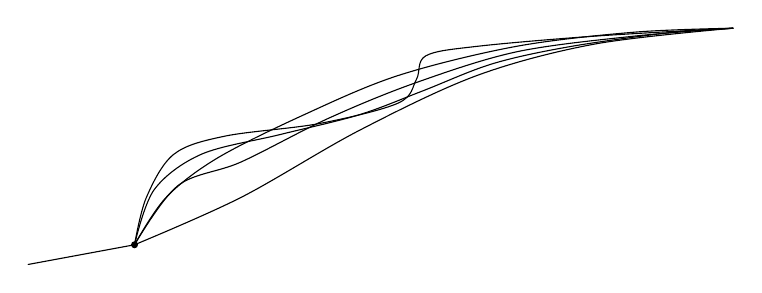
\begin{tikzpicture}[x=1mm,y=1mm,line cap=round,line join=round,font=\scriptsize]
\draw (3,-30.5) -- (16.5,-28);
\draw plot[smooth, tension=0.55] coordinates {(16.5,-28) (30,-22) (45,-13.5) (60,-6.5) (75,-2.5) (92.5,-0.5)};
\draw plot[smooth, tension=0.55] coordinates {(16.5,-28) (20.5,-22) (27,-17) (38,-11.5) (50,-6.5) (65,-2.8) (80,-1) (92.5,-0.5)};
\draw plot[smooth, tension=0.55] coordinates {(16.5,-28) (18,-22) (21.5,-16.5) (28,-14.2) (40,-12.6) (50,-10) (52.3,-7) (53.5,-4) (60,-2.8) (75,-1.5) (92.5,-0.5)};
\draw plot[smooth, tension=0.55] coordinates {(16.5,-28) (19,-21) (25,-16.5) (35,-14) (45,-11.5) (53,-8.5) (62,-5) (72,-2.8) (85,-1) (92.5,-0.5)};
\draw plot[smooth, tension=0.55] coordinates {(16.5,-28) (22,-20.5) (30,-17.5) (41,-12) (52,-7.5) (65,-3.5) (80,-1.5) (92.5,-0.5)};
\node[pt] at (16.5,-28) {};
\end{tikzpicture}
\end{document}
